\section{Análise Léxica}

\begin{frame}[fragile]{{\it Scanners}}

    \begin{itemize}
        \item Em uma dada gramática, as sentenças de uma linguagem são compostas por cadeias de tokens
        \pause

        \item A sequência de caracteres que compõem um único token é denominada lexema
        \pause

        \item Um \textit{scanner} (ou analisador léxico) processa a entrada para produzir uma sequência de tokens
        \pause

        \item Dentre as diferentes tarefas que um \textit{scanner} pode realizar estão: remoção de espaços em branco e comentários, identificação de
            constantes, identificadores e palavras-chave
    \end{itemize}

\end{frame}

\begin{frame}[fragile]{Remoção de espaços em branco e comentários}

    \begin{itemize}
        \item No fluxo de entrada, a presença de outros caracteres que não fazem parte da gramática pode levar a erros no tradutor
        \pause

        \item Várias linguagens permite a presença de ``espaços em branco'' (espaço em branco, nova linha, tabulação, etc) entre os tokens
        \pause

        \item Os espaços em branco podem ser tratados de duas maneiras:
        \pause
        \begin{enumerate}
            \item a gramática deve ser alterada para contemplar os espaços (localização, quantidade, etc), o que traz dificuldades para a especificação da gramática
            e para a implementação do \textit{scanner}
            \pause

            \item o \textit{scanner} simplesmente ignora os espaços em branco (solução mais comum)
        \end{enumerate}
        \pause

        \item O \textit{scanner} também pode ignorar o comentários, de modo que estes possam ser tratados como espaços em branco
    \end{itemize}

\end{frame}

\begin{frame}[fragile]{Identificação de constantes inteiras}

    \begin{itemize}
        \item Constantes inteiras são sequências de dígitos
        \pause

        \item As constantes podem ser inseridas na gramática da linguagem por meio de produções, ou sua identificação pode ser delegada para o analisador léxico,
            que irá criar tokens para estas constantes
        \pause

        \item A segunda alternativa permite tratar constantes inteiras como unidades autônomas durante a tradução
        \pause

        \item Para cada constante inteira, o \textit{scanner} gerará um token e um atributo, sendo o token um identificador de constantes inteiras (por exemplo,
            \code{pascal}{num}) e o atributo o valor inteiro da constante
        \pause

        \item Por exemplo, a entrada \code{cpp}{3 + 14 + 15} seria transformada na sequência de tokens
        \begin{center}
            \code{cpp}{<num, 3>}\ \ \ \ \code{cpp}{<+,>}\ \ \ \ \code{cpp}{<num, 14>}\ \ \ \ \code{cpp}{<+,>}\ \ \ \ \code{cpp}{<num, 15>} 
        \end{center}
        onde o par \code{cpp}{<x, y>} indica que o token \code{cpp}{x} tem atributo \code{cpp}{y}
    \end{itemize}

\end{frame}

\begin{frame}[fragile]{Reconhecimento de identificadores e palavras-chave}

    \begin{itemize}
        \item As linguagens de programação utilizam identificadores para nomear variáveis, vetores, funções e outros elementos
        \pause

        \item As gramáticas das linguagens, em geral, tratam os identificadores como tokens
        \pause

        \item Os analisadores gramaticais (\textit{parsers}) destas gramáticas esperam um mesmo token (por exemplo, \textbf{id}) sempre que um identificador
            aparece na entrada
        \pause

        \item Por exemplo, a expressão \code{cpp}{x = x + y;} deve ser convertida pelo \textit{scanner} para 
        \begin{center}
            \textbf{id} \code{cpp}{=} \textbf{id} \code{cpp}{+} \textbf{id}\code{cpp}{;}
        \end{center}
        \pause

        \item Na análise sintática, é útil saber que as duas primeiras ocorrências de \textbf{id} se referem ao lexema \code{cpp}{x}, enquanto que a última
            se refere ao lexema \code{cpp}{y}
    \end{itemize}

\end{frame}

\begin{frame}[fragile]{Reconhecimento de identificadores e palavras-chave}

    \begin{itemize}
        \item Uma tabela de símbolos pode ser usada para determinar se um dado lexema já foi encontrado ou não
        \pause

        \item Na primeira ocorrência o lexema é armazenado na tabela de símbolos e também nela, e em todas as demais ocorrências, o lexema se torna o atributo
            do token \textbf{id}
        \pause

        \item As palavras-chave da linguagem são cadeias fixas de caracteres usadas como pontuação ou para identificar determinadas construções
        \pause

        \item Em geral, as palavras-chave seguem a mesma regra de formação dos identificadores
        \pause

        \item Se as palavras-chave forem reservadas, isto é, não puderem ser usadas como identificadores, a situação fica facilitada: um lexema só será um
            identificador caso não seja uma palavra-chave
    \end{itemize}

\end{frame}

\begin{frame}[fragile]{Interface para um analisador léxico}

    \begin{figure}
        \centering

        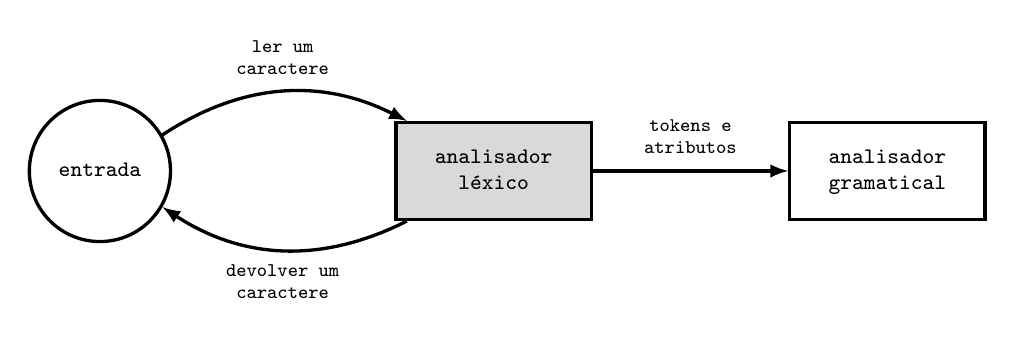
\begin{tikzpicture} 
            \node[circle,draw,very thick] (A) at (0, 0) { \footnotesize \begin{tabular}{>{\tt}c}entrada\end{tabular} };
            \node[fill=gray!30,draw,very thick,inner sep=8pt] (B) at (5, 0) { \footnotesize \begin{tabular}{>{\tt}c}analisador\\ léxico\end{tabular} };
            \node[draw,very thick,inner sep=8pt] (C) at (10, 0) { \footnotesize \begin{tabular}{>{\tt}c}analisador\\ gramatical\end{tabular} };

            \draw[very thick,-latex] (A) to [bend left] node[above] { \scriptsize\begin{tabular}{>{\tt}c}ler um \\ caractere\end{tabular} } (B);
            \draw[very thick,-latex] (B) to node[above] { \scriptsize\begin{tabular}{>{\tt}c}tokens e\\ atributos\end{tabular} } (C);
            \draw[very thick,-latex] (B) to [bend left] node[below] { \scriptsize\begin{tabular}{>{\tt}c}devolver um \\ caractere\end{tabular} } (A);
        \end{tikzpicture} 

    \end{figure}

\end{frame}

\begin{frame}[fragile]{Produtor e consumidor}

    \begin{itemize}
        \item O analisador léxico e o analisador gramatical formam um par produtor-consumidor
        \pause

        \item O analisador léxico produz tokens; o analisador gramatical os consome
        \pause

        \item A interação entre ambos depende do \textit{buffer} que armazena os tokens produzidos: o \textit{scanner} não pode gerar novos tokens se o
            \textit{buffer} está cheio, o \textit{parser} não pode prosseguir se o \textit{buffer} estiver vazio
        \pause

        \item Em geral, o \textit{buffer} armazena um único token
        \pause

        \item Neste caso, o \textit{parser} pode requisitar ao \textit{scanner}, por demanda, a produção de novos tokens
    \end{itemize}

\end{frame}

\begin{frame}[fragile]{Implementação da identificação de constantes inteiras}

    \begin{itemize}
        \item Para que as constantes inteiras possam ser devidamente identificadas no código do \textit{scanner}, é preciso que elas façam parte da
            gramática
        \pause

        \item Por exemplo, a produção do não terminal $fator$ 
        \[
            fator \to \mathbf{digito}\ |\ (expr)
        \]
        pode ser modificada para
        \[
            fator \to (expr)\ |\ \mathbf{num}\ \ \{imprimir(\mathbf{num}.valor)\}
        \]
        \pause

        \item Em relação à implementação, um token deve ser identificador por um par contendo o identificador do token e o seu atributo
    \end{itemize}

\end{frame}

\begin{frame}[fragile]{Exemplo de implementação do terminal $fator$ em C++}
    \inputsnippet{cpp}{1}{20}{codes/fator.cpp}
\end{frame}

\begin{frame}[fragile]{Exemplo de implementação de um scanner de constantes inteiras em C++}
    \inputsnippet{cpp}{1}{13}{codes/scanner.cpp}
\end{frame}

\begin{frame}[fragile]{Exemplo de implementação de um scanner de constantes inteiras em C++}
    \inputsnippet{cpp}{15}{30}{codes/scanner.cpp}
\end{frame}

\begin{frame}[fragile]{Exemplo de implementação de um scanner de constantes inteiras em C++}
    \inputsnippet{cpp}{32}{47}{codes/scanner.cpp}
\end{frame}
